\documentclass[landscape, a4paper]{article}

%!Tex Root = ../main.tex

% ┌────────────┐
% │ Formatting │
% └────────────┘
\usepackage[english]{babel}
\usepackage[top=0cm,bottom=0cm,left=0cm,right=0cm]{geometry}
\usepackage[export]{adjustbox} % use c, l, r for images
\usepackage{csquotes}
\usepackage[parfill]{parskip}
\usepackage{fontspec}
% \usepackage{anyfontsize}
% \usepackage[]{enumitem}

% ┌──────┐
% │ Math │
% └──────┘
\usepackage{amssymb} % for black triangleright, https://tex.stackexchange.com/questions/570303/use-blacktriangleright-as-itemize-label
\usepackage{amsmath}
\usepackage{mathtools} % for \mathclap and 
\usepackage{breqn}

% ┌────────┐
% │ Tables │
% └────────┘
\usepackage{tabularray}
 % \UseTblrLibrary{diagbox}

% ┌────────┐
% │ Images │
% └────────┘
\usepackage{graphicx}
% \usepackage{float} % for the letter H
% \graphicspath{figures/}
\usepackage{subcaption}

% ┌────────┐
% │ Graphs │
% └────────┘
\usepackage{tikzit}
\usepackage{tikz}
\usetikzlibrary{backgrounds}
\usetikzlibrary{arrows}
\usetikzlibrary{shapes,shapes.geometric,shapes.misc}

% this style is applied by default to any tikzpicture included via \tikzfig
\tikzstyle{tikzfig}=[baseline=-0.25em,scale=0.5]

% these are dummy properties used by TikZiT, but ignored by LaTex
\pgfkeys{/tikz/tikzit fill/.initial=0}
\pgfkeys{/tikz/tikzit draw/.initial=0}
\pgfkeys{/tikz/tikzit shape/.initial=0}
\pgfkeys{/tikz/tikzit category/.initial=0}

% standard layers used in .tikz files
\pgfdeclarelayer{edgelayer}
\pgfdeclarelayer{nodelayer}
\pgfsetlayers{background,edgelayer,nodelayer,main}

% style for blank nodes
\tikzstyle{none}=[inner sep=0mm]

% include a .tikz file
\newcommand{\tikzfig}[1]{%
{\tikzstyle{every picture}=[tikzfig]
\IfFileExists{#1.tikz}
  {\input{#1.tikz}}
  {%
    \IfFileExists{./figures/#1.tikz}
      {\input{./figures/#1.tikz}}
      {\tikz[baseline=-0.5em]{\node[draw=red,font=\color{red},fill=red!10!white] {\textit{#1}};}}%
  }}%
}

% the same as \tikzfig, but in a {center} environment
\newcommand{\ctikzfig}[1]{%
\begin{center}\rm
  \tikzfig{#1}
\end{center}}

% fix strange self-loops, which are PGF/TikZ default
\tikzstyle{every loop}=[]


% ┌────────┐
% │ Citing │
% └────────┘
% \usepackage[style=authortitle]{biblatex}
% \addbibresource{./Graph_Theory.bib}
% \usepackage{cleveref}

% ┌──────────┐
% │ Diagrams │
% └──────────┘
% \usepackage{tikz}
% \usetikzlibrary{shadows, backgrounds} % , calc

% ┌──────────────────┐
% │ Multiple columns │
% └──────────────────┘
% \usepackage{multicol}

% ┌────────────────────┐
% │ Code hightligthing │
% └────────────────────┘
% \usepackage{minted}

% ┌────────────────────────┐
% │ Latex Programming Help │
% └────────────────────────┘
\usepackage{etoolbox}
\usepackage{xparse}
% https://tex.stackexchange.com/questions/358292/creating-a-subcounter-to-a-counter-i-created
\usepackage{chngcntr}

% ┌───────────────┐
% │ Pretty Boxes  │
% └───────────────┘
\usepackage{xcolor}
\usepackage{tcolorbox}
\tcbuselibrary{skins,theorems}

% ┌──────────────┐
% │ Pseudo Code  │
% └──────────────┘
\usepackage{pseudo}

% \usepackage{background}
\usepackage{gradient-text}
\usepackage{rotating}

% \newlength\mylen
% \setlength\mylen{\dimexpr\paperwidth/80\relax}
%
% \SetBgScale{1}
% \SetBgAngle{0}
% \SetBgColor{blue!30}
% \SetBgContents{\tikz{\draw[step=\mylen] (-.5\paperwidth,-.5\paperheight) grid (.5\paperwidth,.5\paperheight);}}

% ┌────────────┐
% │ Misc Tools │
% └────────────┘
\usepackage{lipsum}

%!Tex Root = ../main.tex

% ┌────────────┐
% │ Formatting │
% └────────────┘
% \setlength{\parskip}{0.4cm} % space between paragraphs, https://latexref.xyz/bs-par.html

% ┌───────┐
% │ Fonts │
% └───────┘
\usepackage{fontspec}
\newfontfamily\gyre{DejaVu Math TeX Gyre}
% colored bold
% \newcommand\alert[1]{\textcolor{SwitchColor}{\textbf{#1}}}
\newcommand\alert[1]{\textcolor{SwitchColor}{#1}}

% ┌──────────────┐
% │ Pseudo Code  │
% └──────────────┘
\newcounter{algorithm}
\setcounter{algorithm}{0}
\newtcbtheorem[use counter=algorithm]{algorithm}{\color{SecondaryColor}Algorithm}{pseudo/ruled}{alg}
% \newcommand{\ma}[1]{$\mathcal{#1}$}
% \renewcommand{\tt}[1]{{\small\texttt{#1}}}

% ┌────────┐
% │ Colors │
% └────────┘
\definecolor{PrimaryColor}{HTML}{800080}
\definecolor{PrimaryColorDimmed}{HTML}{D6D6F0}
\definecolor{SecondaryColor}{HTML}{006BB6}
\definecolor{SecondaryColorDimmed}{HTML}{E5F0F8}
\definecolor{SwitchColor}{named}{PrimaryColor}
\colorlet{BoxColor}{gray!10!white}

% ┌───────┐
% │ Links │
% └───────┘
\usepackage[allbordercolors=PrimaryColor, pdfborder={0 0 .2}]{hyperref}

% ┌─────────┐
% │ Mindmap │
% └─────────┘
\renewcommand{\labelitemi}{$\textcolor{SwitchColor}{\bullet}$}
\renewcommand{\labelitemii}{$\textcolor{SwitchColor}{\blacktriangleright}$}
\renewcommand{\labelitemiii}{$\textcolor{SwitchColor}{\blacksquare}$}

%!Tex Root = ../main.tex

% ┌─────────┐
% │ Mindmap │
% └─────────┘
\newlength{\leveldistance}
\setlength{\leveldistance}{25cm}

\newenvironment{edges}{\begin{pgfonlayer}{background}\draw [concept connection]}{;\end{pgfonlayer}}
\newcommand{\edge}[2]{(#1) edge (#2)}
\newcommand{\annotation}[2]{\path (#1) -- node[annotation, above, align=center, pos=0.03] {#2} (middle);}

\newenvironment{resettikz}{\pgfsetlayers{nodelayer,edgelayer}\tikzset{every node/.style={fill opacity=1.0, draw opacity=1.0, minimum size=0cm, inner sep=0pt}}}{}

\newenvironment{mindmap}{
	\begin{tikzpicture}[
			auto,
			huge mindmap,
			fill opacity=0.6,
			draw opacity=0.8,
			concept color = PrimaryColorDimmed,
			every annotation/.style={fill=BoxColor, draw=none, align=center, fill = BoxColor, text width = 2cm},
			grow cyclic,
			level 1/.append style = {
					concept color=SecondaryColorDimmed,
					level distance=\leveldistance,
					sibling angle=360/\the\tikznumberofchildren,
					% https://tex.stackexchange.com/questions/501240/trying-to-use-the-array-environment-inside-a-tikz-node-with-execute-at-begin-no
					execute at begin node=\definecolor{SwitchColor}{named}{SecondaryColor}\definecolor{SwitchColorDimmed}{named}{PrimaryColorDimmed},
				},
			level 2/.append style = {
					concept color=PrimaryColorDimmed,
					level distance=\leveldistance / 2,
					sibling angle=35,
					execute at begin node=\definecolor{SwitchColor}{named}{PrimaryColor}\definecolor{SwitchColorDimmed}{named}{SecondaryColorDimmed},
				},
			level 3/.append style = {
					concept color=SecondaryColorDimmed,
					level distance=\leveldistance / 3,
					execute at begin node=\definecolor{SwitchColor}{named}{SecondaryColor}\definecolor{SwitchColorDimmed}{named}{PrimaryColorDimmed},
				},
			level 4/.append style = {
					concept color=PrimaryColorDimmed,
					level distance=\leveldistance / 4,
					execute at begin node=\definecolor{SwitchColor}{named}{PrimaryColor}\definecolor{SwitchColorDimmed}{named}{SecondaryColorDimmed},
				},
			level 5/.append style = {
					concept color=SecondaryColorDimmed,
					level distance=\leveldistance / 5,
					execute at begin node=\definecolor{SwitchColor}{named}{SecondaryColor}\definecolor{SwitchColorDimmed}{named}{PrimaryColorDimmed},
				},
			level 6/.append style = {
					concept color=PrimaryColorDimmed,
					level distance=\leveldistance / 6,
					execute at begin node=\definecolor{SwitchColor}{named}{PrimaryColor}\definecolor{SwitchColorDimmed}{named}{SecondaryColorDimmed},
				},
			level 7/.append style = {
					concept color=SecondaryColorDimmed,
					level distance=\leveldistance / 7,
					execute at begin node=\definecolor{SwitchColor}{named}{SecondaryColor}\definecolor{SwitchColorDimmed}{named}{PrimaryColorDimmed},
				},
			level 8/.append style = {
					concept color=PrimaryColorDimmed,
					level distance=\leveldistance / 8,
					execute at begin node=\definecolor{SwitchColor}{named}{PrimaryColor}\definecolor{SwitchColorDimmed}{named}{SecondaryColorDimmed},
				},
			level 9/.append style = {
					concept color=SecondaryColorDimmed,
					level distance=\leveldistance / 9,
					execute at begin node=\definecolor{SwitchColor}{named}{SecondaryColor}\definecolor{SwitchColorDimmed}{named}{PrimaryColorDimmed},
				},
			concept connection/.append style = {
					color = BoxColor,
				},
		]
		}{
	\end{tikzpicture}
}

\newenvironment{mindmapcontent}{
	\begin{scope}[
			every node/.style = {concept, circular drop shadow}, % draw=none
			every child/.style={concept},
		]
		}{
		;\end{scope}
}

% ┌───────┐
% │ Boxes │
% └───────┘
\DeclareTotalTCBox{\inlinebox}{ s m }
{standard jigsaw,opacityback=0,colframe=SwitchColor,nobeforeafter,tcbox raise base,top=0mm,bottom=0mm,
	right=0mm,left=0mm,arc=0.1cm,boxsep=0.1cm}
{\IfBooleanTF{#1}%
	{\textcolor{PrimaryColor}{\setBold >\enspace\ignorespaces}#2}%
	{#2}}

\DeclareTotalTCBox{\inlineboxtwo}{ s m }
{standard jigsaw,opacityback=0,colframe=SwitchColorDimmed,nobeforeafter,tcbox raise base,top=0mm,bottom=0mm,
	right=0mm,left=0mm,arc=0.1cm,boxsep=0.1cm}
{\IfBooleanTF{#1}%
	{\textcolor{SwitchColorDimmed}{\setBold >\enspace\ignorespaces}#2}%
	{#2}}

% ┌──────────────────┐
% │ Case distinction │
% └──────────────────┘
% \newtoggle{absolute}
% % \toggletrue{absolute}
% \togglefalse{absolute}
% \newcommand{\lpathgraph}[1]{\iftoggle{absolute}{/home/areo/Documents/Studium/Summaries/x/}{./}#1}

% ┌───────┐
% │ Fixes │
% └───────┘
% https://tex.stackexchange.com/questions/89467/why-does-pdftex-hang-on-this-file
% \newcommand{\colon}{\mathrel{\mathop:}}

% ┌───────┐
% │ Paths │
% └───────┘
% \newcommand{\script}[2]{\href[page=#1]{}{\inlinebox{#2}}}
\newcommand{\script}[2]{\href{openpdf:/home/areo/Documents/Studium/Semester_1_Master/Hardware_Security_and_Trust/slides/Slides annotated/Hardware_Security_and_Trust_all_in_one.pdf:#1}{\inlinebox{#2}}}
\newcommand{\scripttwo}[2]{\href{openpdf:///home/areo/Documents/Studium/Semester_1_Master/Hardware_Security_and_Trust/slides/Slides annotated/bonus/12_Lecture_06Dec.pdf:#1}{\inlinebox{#2}}}
\newcommand{\videoeight}[2]{\href{https://youtu.be/YcHSlFjcndU?feature=shared&t=#1}{\inlineboxtwo{#2}}}
\newcommand{\videonine}[2]{\href{https://youtu.be/3dL-3EOIfJ8?si=l3OakqHOeCpnNayw&t=#1}{\inlineboxtwo{#2}}}
\newcommand{\videoten}[2]{\href{https://youtu.be/6oF737pa510?feature=shared&t=#1}{\inlineboxtwo{#2}}}
\newcommand{\videoeleven}[2]{\href{https://youtu.be/PJTqfzTIYJs?feature=shared&t=#1}{\inlineboxtwo{#2}}}
\newcommand{\videotwelve}[2]{\href{https://youtu.be/oDxAH7aO-Tk?feature=shared&t=#1}{\inlineboxtwo{#2}}}
\newcommand{\videothirteen}[2]{\href{https://youtu.be/3TkSXxe_Ty8?feature=shared&t=#1}{\inlineboxtwo{#2}}}
\newcommand{\videofourteen}[2]{\href{https://youtu.be/1Y3dZuJ0MHg?feature=shared&t=#1}{\inlineboxtwo{#2}}}


\begin{document}
\fontsize{3pt}{3pt}\selectfont

\begin{minipage}[t]{0.2\linewidth}
	\fbox{General} \lecturenotes{/home/areo/Documents/Studium/Semester_2_Master/Program_Verification/slides/bonus/1._Introduction.md} \additionalslides{/home/areo/Documents/Studium/Semester_2_Master/Program_Verification/slides/bonus/1._Introduction.pdf}
	\begin{betterlist}
		\item \alert{Program Verifier:} Takes program and specification and determines whether the program satisfies or if it violates the specification. Tells that in all executions of program specification holds. Also want indication of how specification is violated (i.e. counter example, e.g. inputs to violate assert statement) and also in case of yes want proof, because the program verifier itself could have a bug. \underline{Typical specifications:} No division by zero, Array only accessed within its bounds, Termination, Memory safety, No assert statement is violated
		\item \href{https://ultimate-pa.org/?ui=tool&tool=automizer}{Ultimate Automizer}
		\item \underline{Challenges:}
		\begin{enumerate}
			\item \alert{Undecidability:} The program verification problem is undecidable. There's no algorithm that verify the program and always hold (\underline{compromise:} verification algorithm that always tells correct resutl when it terminates but may not terminate or algorithm that sometimes terminates and says it could not prove the program). \underline{Solution:} Do not try to develop algorithms that solve the problem for all programs. Algorithms that solve the problem for some programs are also helpful.
			\item \alert{Ambiguities:} Different programming languages disagree what should happen for a piece of code. \underline{Solution:} Use mathematical logic to give programming languages a precise semantics
			\item \alert{Correctness Proofs are Hard to Find:} We cannot track all executions.
		\end{enumerate}
	\end{betterlist}
	\fbox{Propositional Logic (PL)} \lecturenotes{/home/areo/Documents/Studium/Semester_2_Master/Program_Verification/slides/bonus/2._Propositional_Logic.md} \additionalslides{/home/areo/Documents/Studium/Semester_2_Master/Program_Verification/slides/bonus/2._Propositional_Logic.pdf}
	\begin{betterlist}
		\item \script{29}{Syntax} and \script{31}{Semantics}, \script{32}{Examples}
		\begin{betterlist}
			\item \alert{Abbreviations:} $true := \neg false$, $(F_1 \lor F2 ) := \neg (\neg F_1 \land \neg F2)$, $(F_1 \rightarrow F2) := (\neg F_1 \lor F2)$, $(F_1 \leftrightarrow F2) := ((F_1 \rightarrow F2) \land (F2 \rightarrow F_1))$
			\item \underline{Terminology:} We call true, false \alert{atoms}, If $X \in V_{PL}$, we call $X$ an \alert{atom}, If $F$ is an atom, we call $F$ and $\neg F$ a \alert{literal}, We call the symbols $\neg$, $\wedge$, $\vee$, $\rightarrow$, $\leftrightarrow$ \alert{logical connectives}
			\item order of \alert{precedence} for logical connectives: $\neg, \land, \lor, \rightarrow, \leftrightarrow$. Binary operators are \alert{right-associative} ($F_1 \rightarrow F_2 \rightarrow F_3$ is $F_1 \rightarrow (F_2 \rightarrow F_3 )$)
		\end{betterlist}
		\item We call a PL formula $F$ \alert{satisfiable} if there is a variable assignment $\rho$ such that the evaluation $[[F]]_\rho$ is true. Otherwise, we say that $F$ is \alert{unsatisfiable}. We call a PL formula $F$ \alert{valid} if for all variable assignments $\rho$ the evaluation $[[F]]\rho$ is true
		\begin{betterlist}
			\item Deciding \alert{satisfiability} of a PL formula is an \alert{NP-complete} problem. \alert{Truth table} has problem of limited applicability, because a truth table has one row per variable assignment, and there are $2^n$ (exponential) variable assignments for $n$ variables. There are many algorithms that work well in practice and that are known to be \alert{polynomial} on relevant \alert{subclasses of PL formulas}. \alert{SAT solver} for propositional logic. \alert{SMT solver} (satisfiability modulo theories) for first order logic modulo theories
		\end{betterlist}
		\item Let $\Gamma = \{F_1, \ldots F_n\}$ be a set of PL formulas, and let $F′$ be another PL formula $F′$. We say that $\Gamma$ \alert{entails} $F'$ if for all variable assignments $\rho$ we have that if $[[F_i]]\rho = true$ holds for all $i \in \{1, \ldots n\}$, then also $[[F′]]\rho = true$ holds. We use $\models$ to denote this entailment relation and we say that the entailment $\Gamma \models F′$ holds if $\Gamma$ entails $F′$. \script{38}{Examples}. Prove that $\{F_1, \ldots F_n\}$ entails $F′$:
		\begin{betterlist}
			\item truth table (Not doable if number of variables is high)
			\item prove that the PL formula $F_1 \land \ldots \land F_n \rightarrow F′$ is valid (Requires algorithm for checking validity)
			\item prove that the PL formula $\neg(F_1 \land . . . \land F_n \rightarrow F′)$ is not satisfiable (Requires algorithm for checking satisfiability, implemented in SMT solvers)
			\begin{betterlist}
				\item the PL formula $F$ is valid iff the PL formula $\neg F$ is unsatisfiable. \script{39}{Proof}
			\end{betterlist}
			\item proof system
		\end{betterlist}
		\item We call two PL formulas $F_1$ and $F_2$ \alert{equivalent}, denoted $F_1 \equiv F_2$, if they evaluate to the same truth value under each variable assignment. $F_1 \equiv F_2 \text{iff} \{F_1\} \models F_2 \text{and} \{F_2\} \models F_1$
	\end{betterlist}
	\fbox{PL Proof system ($N_{PL}$)}
	\begin{betterlist}
		\item proof system for deriving valid PL entailments $\Gamma \models F$
		\item template for giving a proof. Reasoning according to a fixed number of rules. Prove once that every rule is \enquote{correct}. Check a proof $\leadsto$ check if every step is an instance of a rule. Find a proof $\leadsto$ find a sequence of rules
		\item $\mathcal{N}_{PL}$: Proof system for entailments between PL formulas. Proof rules are $(n + 1)$-ary relations over entailments denoted as: $\frac{\Gamma_1 \vDash F_1 \quad \ldots \quad \Gamma_n \vDash F_n}{\Gamma_{n+1} \vDash F_{n+1}}$.  If $\Gamma_i$ entails $F_i$ for all $i \in \{1, \ldots n\}$, then $\Gamma_{n+1}$ entails $F_{n+1}$
		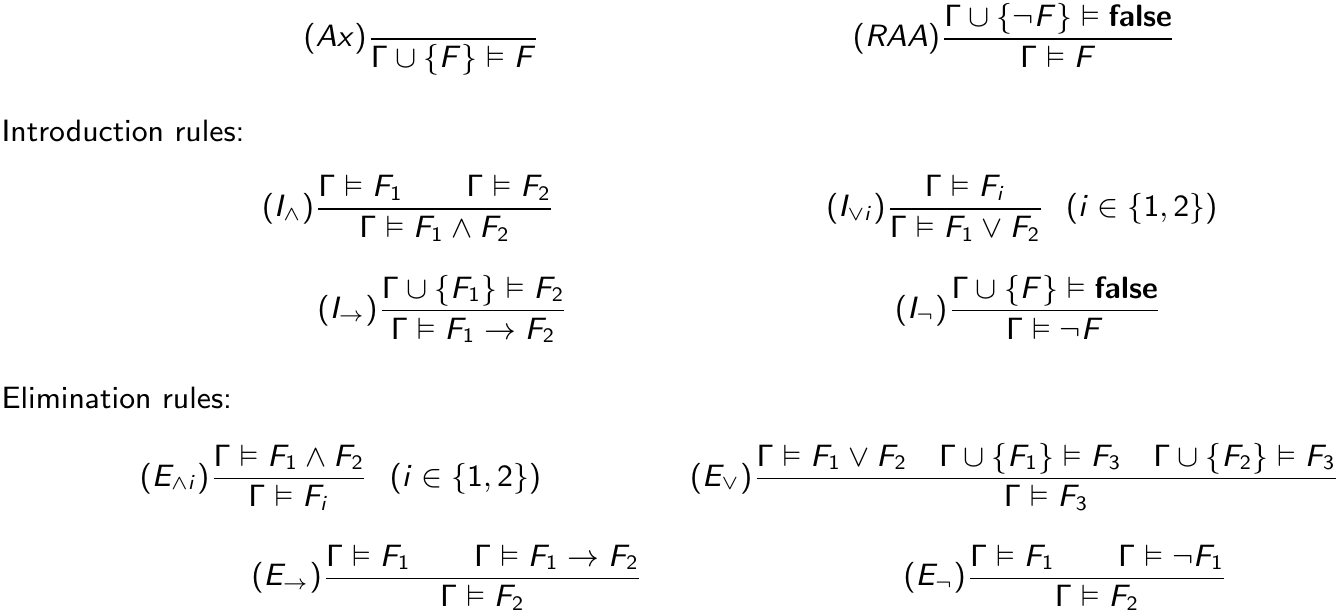
\includegraphics[width=0.7\linewidth]{./figures/proof_rules.png}  (called inference rules)
		\begin{betterlist}
			\item can find a derivation and conclude that the entailment holds
		\end{betterlist}
		\item A \alert{derivation} is a tree whose nodes are labelled by entailments such that the following holds: If a node labelled by entailment $\Gamma_{n+1} \models F_{n+1}$ has children that are labelled by entailments $\Gamma_1 ⊨ F_1 \ldots \Gamma_n ⊨ F_n$, then $\frac{\Gamma_1 \vDash F_1 \quad \ldots \quad \Gamma_n \vDash F_n}{\Gamma_{n+1} \vDash F_{n+1}}$ must be an instance of some rule. \script{44}{Example}. \script{45}{Remarks (f.)}
		\begin{betterlist}
			\item  \script{48}{Example: Construction of a Derivation}, \script{49}{Guide for proving entailments (f.)}
		\end{betterlist}
		\item \alert{Theorem (Soundness of $N_{PL}$):} If a node in a derivation is labelled by $\Gamma \models F$, then the entailment $\Gamma \models F$ holds. \script{47}{Proof}
		\item \alert{Theorem (Completeness of $N_{PL}$):} If the entailment $\Gamma \models F$ holds, then there exists a derivation where the root is labelled by $\Gamma \models F$
	\end{betterlist}
	\fbox{First-Order Logic (FOL)}
	\begin{betterlist}
		\item \script{56}{Examples (f.)}
		\item \underline{syntax:} \script{58}{Vocabulary and Terms}, \script{59}{Formulas}
		\begin{betterlist}
			\item $\forall x:\phi) := \neg(\exists x:\neg\phi)$, abbreviate $\exists x1 .\exists x2 .\phi$ to $\exists x1 , x2 .\phi$ and similarly for $\forall$
			\item \alert{quantifiers:}$\exists$ and $\forall$. \alert{atoms:} $true$, $false$, and $p(t_1, \ldots, t_n)$
			\item \alert{precedence} of quantifiers is lower than the precedence of logical connectives
			\item \script{60}{Model and $f \triangleleft \{\tilde{x}\rightarrow \tilde{y}\}$ notation}
			\item \underline{evaluation:} \script{61}{of terms} and \script{62}{of  formulas}
		\end{betterlist}
		\item we call a formula $\varphi$ \alert{satisfiable} if there exists a model $M$ and a variable assignment $\rho$ such that $[[\varphi]]_{M,\rho} = true$. Otherwise, $\varphi$ is \alert{unsatisfiable}. We call a formula $\varphi$ \alert{valid} if $[[\varphi]]_{M,\rho} = true$ for all models $M$ and for all variable assignments $\rho$
		\begin{betterlist}
			\item $\varphi$ is valid iff $\neg \varphi$ is unsatisfiable
		\end{betterlist}
		\item given a (possibly infinite) set of FOL formulas $\Gamma$ and a FOL formula $\psi$, we say that $\Gamma$ \alert{entails} $\psi$ if for all models $M$ and for all variable assignments $\rho$ we have that if $[[\phi]]_{M,\rho} = true$ holds for all $\phi \in \Gamma$ then also $[[\psi]]_{M,\rho} = true$ holds
		\begin{betterlist}
			\item we use $\models$ to denote this entailment relation and we say that \alert{the entailment $\Gamma \models \psi$ holds} if $\Gamma$ entails $\psi$
		\end{betterlist}
		\item \script{66}{Free Variables, Bound Variables, Closed Formulas}
		\item \script{67}{Substitution}
		\begin{betterlist}
			\item \underline{notation:}
			\begin{betterlist}
				\item given a function $f$, we use $dom(f)$ to denote the domain of $f$. Given a function $f$ that maps variables to terms, we use $vars(f)$ to denote the set that contains $dom(f)$ and all variables of all terms in the range of $f$. I.e., $\displaystyle vars(f) = dom(f) \cup \bigcup_{x\in dom(f)} freevars(f(x))$
				\item if we do not want to specify the substitution function $\sigma$ separately, we write $\varphi[x_1 \mapsto t_1, \ldots, x_n \mapsto t_n ]$ instead of $\varphi\sigma$ if $\sigma$ is the function that maps $x_i$ to $t_i$ for $i \in \{1, \ldots , n\}$.
				\item we sometimes use $\varphi[x]$ to refer to a formula and a variable. We may then use in this context $\varphi[t]$ to denote $\varphi[x \mapsto t]$
			\end{betterlist}
		\end{betterlist}
	\end{betterlist}
	\fbox{FOL Proof system ($N_{FOL}$)}
	\begin{betterlist}
		\item proof system for deriving valid FOL entailments $\Gamma \models \varphi$
		\item $N_{FOL}$ (natural deduction for first order logic):

		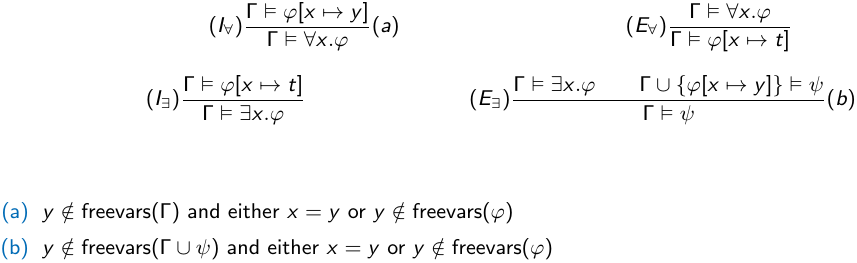
\includegraphics[width=0.7\linewidth]{./figures/nfol.png}
		\begin{betterlist}
			\item two of these rules have additional \alert{side conditions} that are written right beneath the rule. A tree is only a \textit{derivation} if all side conditions are satisfied. \script{72}{All rules}
		\end{betterlist}
		\item \underline{derivation:} \script{71}{Example}
		\begin{betterlist}
			\item use derivation (this tree) as a proof
		\end{betterlist}
		\item \script{80}{When use infix notation}
	\end{betterlist}
	\fbox{First-Order Theories}
	\begin{betterlist}
		\item \script{81}{Motivation (pr.)}
		\item \alert{first-order theory T} consists of:
		\begin{betterlist}
			\item a signature $\Sigma$ - set of constant, function, and predicate symbols
			\item a set of axioms $A_T$ - set of closed (no free variables) $\Sigma$-formulae
		\end{betterlist}
		\item a \alert{$\Sigma$-formula} is a formula constructed of constants, functions, and predicate symbols from $\Sigma$, and variables, logical connectives, and quantifiers
		\item \underline{idea:} the symbols of $\Sigma$ are just symbols without prior meaning. The axioms of $T$ provide their meaning
		\item \alert{$T$-model:} a model $M$ is a \alert{$T$ -model}, if $[[\varphi]]_{M,\rho} = true$ for all $\varphi \in A_T$ and for all variable assignments $\rho$
		\item \alert{$T$-valid:} a $\Sigma$-formula $\varphi$ is \alert{valid in theory $T$} (\alert{$T$ -valid}), if for every $T$ -model $M$ and variable assignment $\rho$, it holds that $[[\varphi]]_{M,\rho} = true$
		\item \alert{$T$-satisfiable:} a $\Sigma$-formula $\varphi$ is \alert{satisfiable} in $T$ (\alert{$T$ -satisfiable}), if there is a $T$ -model $M$ and variable assignment $\rho$ such that $[[\varphi]]_{M,\rho} = true$
		\item \alert{$T$-equivalent:} two $\Sigma$-formulae $\varphi_1$ and $\varphi_2$ are \alert{equivalent in $T$} (\alert{$T$ -equivalent}), if $\varphi_1 \leftrightarrow \varphi_2$ is $T$ -valid
		\item \script{90}{\alert{Axiom Schemata}}
	\end{betterlist}
\end{minipage}
\begin{minipage}[t]{0.2\linewidth}
	\fbox{Collection of First-Order Theories and their decidability} \lecturenotes{/home/areo/Documents/Studium/Semester_2_Master/Program_Verification/slides/bonus/06._First_Order_Theories.md} \additionalslides{/home/areo/Documents/Studium/Semester_2_Master/Program_Verification/slides/bonus/06._First_Order_Theories.pdf}
	\begin{betterlist}
		\item \script{89}{Theory of Equality (pr.)}, \script{93}{Theory of Rock-Paper-Scissors (pr.)}
		\item \alert{Decidability}: We call a problem \alert{decidable} if there exists an algorithm that terminates on all instances of the problem and gives a correct yes/no answer.
		\begin{betterlist}
			\item \uline{example undecidable problem:} Halting Problem for Turing machines, \uline{prove decidability:} give an algorithm and prove its correctness, \uline{prove undecidability:} reduction from a known undecidable problem
			\item \alert{Satisfiability} of PL formulas is \alert{decidable}, \alert{Satisfiability} of FOL formulas is \alert{undecidable}
			\item \alert{$T_{E}$-validity} is \alert{undecidable}, For a \alert{quantifier-free formula $T_E$-validity} is \alert{decidable}
			\item \script{100}{Peano Arithmetic $T_{PA}$ (first-order arithmetic) (ff.)}: natural numbers with addition and multiplication
			\begin{betterlist}
				\item \script{101}{Definition of $\le$ etc.}, \script{102}{$EXP[x, n, r]$}
				\item \alert{$T_{PA}$} is \alert{undecidable}, \alert{quantifier-free fragment of $T_{PA}$} is \alert{undecidable}
				\item \script{103}{\alert{Gödel’s first incompleteness theorem}}: \uline{Peano arithmetic $T_{PA}$ does not capture true arithmetic:} There exist closed $\Sigma_{PA}$-formulae representing valid propositions of number theory that are not $T_{PA}$-valid. \uline{The reason:} $T_{PA}$ actually admits nonstandard interpretations. \underline{For decidability:} \alert{no multiplication}
			\end{betterlist}

			\item \script{104}{Presburger Arithmetic $T_{\mathbb{N}}$}: natural numbers with addition
			\begin{betterlist}
				\item \alert{$T_{\mathbb{N}}$-satisfiability} and \alert{$T_{\mathbb{N}}$-validity} are \alert{decidable}
			\end{betterlist}
			\item \script{106}{Theory of Integers $T_{\mathbb{Z}}$ (pr.)}: integers with $+$, $−$, $>$
			\begin{betterlist}
				\item \alert{$T_{\mathbb{Z}}$-satisfiability} and \alert{$T_{\mathbb{Z}}$-validity} are \alert{decidable}
			\end{betterlist}
			\item \script{108}{Theory of Arrays $T^=_A$ (with extensionality)}, \script{109}{Theory of Bit-vectors (f.)}, \script{111}{Theory of Floats}
			\item \script{113}{Overview decidability}
		\end{betterlist}
	\end{betterlist}
	\fbox{SMT-LIB} \lecturenotes{/home/areo/Documents/Studium/Semester_2_Master/Program_Verification/slides/bonus/07._Boogie_and_Boostan.md} \additionalslides{/home/areo/Documents/Studium/Semester_2_Master/Program_Verification/slides/bonus/07._Boogie_and_Boostan.pdf}
	\begin{betterlist}
		\item \script{117}{What it is}, \script{118}{SMT Script}, \script{119}{Theories}, \script{122}{Logics (f.)}
		\item \script{124}{Terms definined in lecture and SMT-LIB (pr.)}, \script{126}{Terms (pr.)}
		\item \script{127}{Links to solvers}
		\item \script{129}{Commands (pr.)}
	\end{betterlist}
	\fbox{Boogie and Boostan Syntax}
	\begin{betterlist}
		\item \script{138}{Boogie and Boogaloo (prr.)}, \script{139}{Examples (f.)}, \script{141}{Options}
		\item \script{142}{Boostan}
		\item \script{146}{Context-free grammar}, \script{147}{Derivation tree}, \script{148}{Derived word}
		\item \script{152}{Grammar for Numbers}, \script{153}{Grammar for Variables}, \script{154}{Grammar for Integer Expressions}, \script{156}{Grammar for Boolean Expressions}, \script{157}{Grammar for Statements}
		\begin{betterlist}
			\item \underline{we call}: A subword that is derived from $X_{var}$ a (program) \alert{variable}, A subword that is derived from $X_{iexpr}$ or $X_{bexpr}$ an \alert{expression}, A subword that is derived from $X_{stmt}$ a (program) \alert{statement}
		\end{betterlist}
	\end{betterlist}
	\fbox{(Boogie and) Boostan Semantics}
	\begin{betterlist}
		\item \script{159}{Boostan program}
		\item \script{161}{Problem with C Semantics (ff.)}
		\item \script{167}{Relational semantics (f.)}
		\item \script{169}{Program State}, \script{179}{Set of states} (\script{170}{Sets of Program States (first mentioned)})
		\item \script{171}{Semantics of Expressions}
		\begin{betterlist}
			\item \underline{idea:} Assign each expression an SMT formula. Given an expression $expr$, we define the semantics of the expression, denoted $[[expr]]$ as the SMT formula that is denoted by the same string
			\item \script{171}{Exceptions}
			\item \script{179}{Convention: Omit double brackets} (\script{171}{Convention $expr$ instead of $[[expr]]$} (first mentioned))
		\end{betterlist}
		\item \script{172}{Semantics of the Assignment Statement (f.)}
		\item \script{178}{Semantics of the Concatenation of Statements}
		\begin{betterlist}
			\item \script{177}{Relational Composition}
		\end{betterlist}
		\item \script{180}{Semantics of the If-then-else Statement}
		\item \script{183}{Semantics of the While Statement}
		\begin{betterlist}
			\item \script{181}{Reflexive Transitive Closure} and \script{182}{Example}
		\end{betterlist}
		\item \script{184}{Full Example (f.)}
	\end{betterlist}
	\fbox{Hoare Proof System}
	\begin{betterlist}
		\item proof system for deriving valid Hoare triples $\{\varphi\} st \{\psi\}$
		\item a program $P$ \alert{satisfies the precondition-postcondition pair} $(\{\varphi_{pre}\}, \{\varphi_{post}\})$ if the inclusion $post(\{\varphi_{pre}\}, [[st]]) \subseteq \{\varphi_{post}\}$ holds (\script{189}{Precondition-Postcondition Pairs})
		\begin{betterlist}
			\item given a binary relation $R$ over the set $X$ and a subset of $Y \subseteq X$, the \alert{postimage of $Y$ under $R$},
			denoted $post(Y , R)$, is the set $\{x \in X \mid \text{ exists } y \in Y \text{ such that } (y, x) \in R\}$. \script{190}{Example}
			\item \script{191}{Full Example}
		\end{betterlist}
		\item given a set of states $\{\varphi\}$, a program statement $st$ and a set of states $\{\psi\}$, we call the triple $\{\varphi\} st \{\psi\}$ a \alert{Hoare triple}
		\item we call a Hoare triple $\{\varphi\} st \{\psi\}$ \alert{valid} if $st$ satisfies the precondition-postcondition pair $(\{\varphi\}, \{\psi\})$. \script{197}{Example}
		\item \underline{\script{200}{Rules}:}

		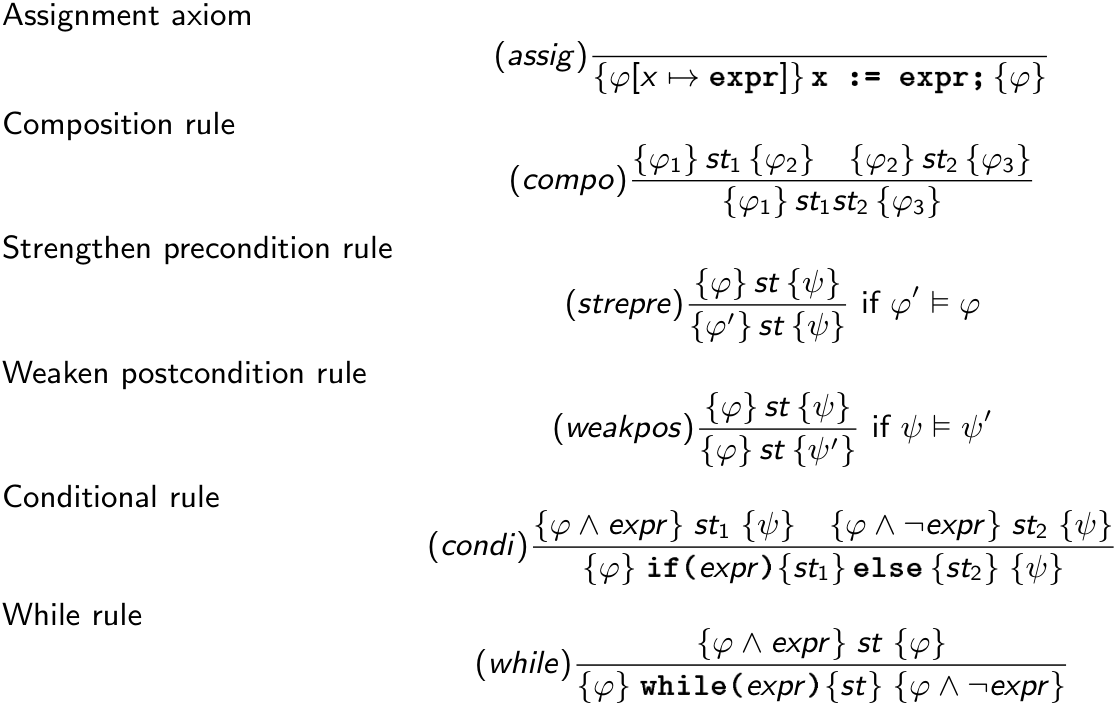
\includegraphics[width=0.7\linewidth]{./figures/hoare_rules.png}
		\begin{betterlist}
			\item \script{202}{Example: Assignment axiom}
			\item \script{203}{Example: Conditional Rule}
			\item \script{204}{Example: While Rule}
			\item \script{205}{Full Example}
		\end{betterlist}
		\item we define a \alert{derivation} as a tree whose nodes are labelled by Hoare triples such that the following holds. If a node that is labelled by a Hoare triple $\{\varphi_{n+1}\} st_{n+1} \{\psi_{n+1}\}$ has children that are labelled by Hoare triples $\{\varphi_1\} st_1 \{\psi_1\} \ldots \{\varphi_n\} st_n \{\psi_n\}$, then the following must be an instance of some rule: $\frac{\{\varphi_1\} st_1 \{\psi_1\} \ldots \{\varphi_n\} st_n \{\psi_n\}}{\{\varphi_{n+1}\} st_{n+1} \{\psi_{n+1}\}}$ (\script{201}{Derivation in context hoare proof system})
		\item \alert{Soundness of the Hoare Proof System:} If there is a derivation whose root is labelled by $\{φ\} st \{ψ\}$, then the statement $st$ satisfies the precondition-postcondition pair $(\{φ\}, \{ψ\})$
		\begin{betterlist}
			\item we call a rule of the form $\frac{\{\varphi_{1}\} st_{1} \{\psi_{1}\} \ldots \{\varphi_{n}\} st_{n} \{\psi_{n}\}}{\{\varphi_{n+1}\} st_{n+1} \{\psi_{n+1}\}}$ \alert{sound} if the following holds: If for all $i \in\{1, \ldots, n\}$ the Hoare triple ${\varphi_i} st_i {\psi_i}$ is valid, then the Hoare triple ${\varphi_{n+1}} st_{n+1} {\psi_{n+1}}$ is also valid. (\script{209}{Sound rule})
			\item \script{210}{Soundness of the Assignment Axiom}
			\item \script{211}{Soundness of the Composition Rule}
			\item \script{212}{Soundness of the Strengthen Precondition Rule}
			\item \script{213}{Soundness of the Weakening Postcondition Rule}
			\item \script{214}{Soundness of the Conditional Rule}
			\item \script{215}{Soundness of the While Rule (ff.)}
			\item \script{218}{Soundness of the Hoare Proof System (f.)}
		\end{betterlist}
	\end{betterlist}
	\fbox{Boostan Extended Syntax}
	\begin{betterlist}
		\item \script{242}{Arrays}
		\begin{betterlist}
			\item \script{243}{SMT-LIB}
			\item \script{244}{Memory via Arrays}
			\item \script{249}{Grammar}
		\end{betterlist}
		\item \script{255}{Havoc Statement (f.)}
		\begin{betterlist}
			\item \href{https://www.microsoft.com/en-us/research/wp-content/uploads/2016/12/krml178.pdf}{\inlinebox{Section 9.4 of Specification}}
			\item \script{258}{Grammar}
		\end{betterlist}
		\item \script{264}{Assume Statement}
		\begin{betterlist}
			\item \href{https://www.microsoft.com/en-us/research/wp-content/uploads/2016/12/krml178.pdf}{\inlinebox{Section 9.2 of Specification}}
			\item \script{266}{Grammar}
		\end{betterlist}
	\end{betterlist}
	\fbox{Boostan Extended Semantics}
	\begin{betterlist}
		\item \script{250}{Arrays}
		\item \script{259}{Havoc Statement}
		\item \script{267}{Assume Statement}
	\end{betterlist}
	\fbox{Hoare Proof System Extended}
	\begin{betterlist}
		\item \underline{Rules:}

		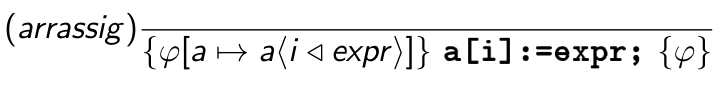
\includegraphics[width=0.5\linewidth]{./figures/arrassig.png}

		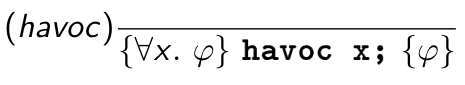
\includegraphics[width=0.325\linewidth]{./figures/havoc.png}

		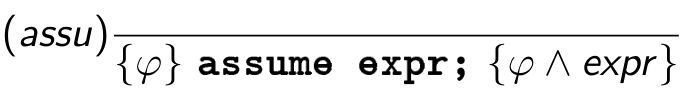
\includegraphics[width=0.4\linewidth]{./figures/assu.png}
		\begin{betterlist}
			\item \script{252}{Soundness of the Array Assignment Axiom}
			\item \script{261}{Soundness of the Havoc Axiom}
			\item \script{269}{Soundness of the Assume Axiom}
		\end{betterlist}
	\end{betterlist}
\end{minipage}
\begin{minipage}[t]{0.2\linewidth}
	\fbox{Ultimate Referee}
	\begin{betterlist}
		\item \script{227}{Guide for Finding a Derivation in the Hoare Proof System}
		\item \script{230}{What it is and example (ff.)}
		\item \script{233}{Interactive verification, Deductive verification, Automated verification}
	\end{betterlist}
	\fbox{Control-flow graphs}
	\begin{betterlist}
		\item \script{279}{Control-Flow Graph}, \script{279}{Control-Flow Graph for a Program}, \script{280}{Example}
		\begin{betterlist}
			\item \underline{useful for automated verification:} apply algorithms from graph theory / automata theory
			\item captures only one aspect of a program, it defines the way in which the programmer arranged the statements in the code
			\item focused solely on the program’s data but it is not sufficient to specify the situation in which a program currently is, because the state does not provide information about the next statements that can be executed
			\item \script{281}{Notational Conventions}
			\item all control-flow graphs for a given statement are \alert{isomorphic} to each other
		\end{betterlist}
		\item \script{282}{Sequential Composition}, \script{283}{Example}
		\item \script{284}{Conditional Statement}, \script{285}{Example}
		\item \script{286}{While Statement}, \script{287}{While Statement}
		\item we call a pair $(\ell, s)$ a \alert{program configuration} of $P$ if $\ell \in Loc$ is a location and $s$ is a state of $P$
		\item we call a sequence of program configurations $(\ell_0, s_0), . . . , (\ell_n, s_n)$ an \alert{execution} of $P$ if there exists a sequence of statements $st_1 \ldots st_n$ such that for each $i \in \{0, \ldots, n−1\}:$ $(\ell_i, st_{i+1}, \ell_{i+1}) \in \Delta$and $(s_i, s_{i+1}) \in [[st_{i+1}]]$. \script{292}{Example}
		\begin{betterlist}
			\item Executions do not have to start at the initial location and do not have to end at the exit location
		\end{betterlist}
		\item we call the program configuration $(\ell, s)$
		\begin{betterlist}
			\item \alert{initial}, if $\ell= \ell_{init}$ and $s \in\{\varphi_{pre}\}$
			\item an \alert{error configuration} if $\ell= \ell_{ex}$ and $s \not\in \{\varphi_{post}\}$
		\end{betterlist}
		\item \alert{Theorem PppSatAndExec:} The program $P = (V, \mu, st)$ satisfies the precondition-postcondition pair $(\varphi_{pre}, \varphi_{post})$ iff there exists no execution $(\ell_0, s_0), \ldots, (\ell_n, s_n)$ such that $(\ell_0, s0)$ is an initial configuration and $(\ell_n, sn)$ is an error configuration
		\begin{betterlist}
			\item so far we only had one way to formally show that $(\varphi_{pre}, \varphi_{post})$ is not satisfied: compute the binary relation over states for this program to check if every pair satisfies the precondition-postcondition pair. By Theorem PppSatAndExec we now have an alternative within our formal setting: we can give an execution
			\item \script{296}{Example program that shows need for Theorem CorrectIffNoErrorReach}
		\end{betterlist}
		\item \alert{Reachable Program Configuration:} We call a configuration $(\ell, s)$ \alert{reachable} if there exists a program execution $(\ell_0, s_0), . . . , (\ell_n, s_n)$ such that $(\ell_0, s_0)$ is an initial configuration and $(\ell_n, s_n) = (\ell, s)$
		\item \alert{Theorem CorrectIffNoErrorReach:} A program satisfies a given precondition-postcondition pair iff the set of reachable configurations does not contain an error configuration
		\item the \alert{set of reachable configurations $RC$} is the smallest set such that
		\begin{betterlist}
			\item each initial configuration is an element of RC
			\item if $(\ell, s) \in RC$, $(\ell, st, \ell') \in \Delta$ and $(s, s′) \in [[st]]$ then $(\ell′, s′) \in RC$
		\end{betterlist}
    \item the \alert{reachability graph} is a pair $(RC, T)$ such that $((\ell, s), st, (\ell′, s′)) \in T$ iff $(\ell, st, \ell') \in \Delta$ and $(s, s′) \in [[st]]$
	\end{betterlist}
\end{minipage}
\begin{minipage}[t]{0.2\linewidth}
\end{minipage}
\begin{minipage}[t]{0.2\linewidth}
\end{minipage}

\newpage

\begin{minipage}[t]{0.2\linewidth}
\end{minipage}
\begin{minipage}[t]{0.2\linewidth}
\end{minipage}
\begin{minipage}[t]{0.2\linewidth}
\end{minipage}
\begin{minipage}[t]{0.2\linewidth}
\end{minipage}
\begin{minipage}[t]{0.2\linewidth}
\end{minipage}
\end{document}
